\section{Sensor Noise}

The wavefront sensor will experience several noise sources that limit the accuracy of the centroid algorithm and the control loop.  Most notably are the discrete sampling of the intensity distribution, the incident photon noise and the detector readout noise.  The latter two are discussed here.  

\subsection{Photon Noise}
Photon noise, also called Shot noise, is due to the stochastic characteristics of light \cite{NumSimCCD2011}.  Photons arrive at the sensor as an average number of events per pixel, with a certain fluctuation in number of arriving pixels.  This noise will vary with the exposure time and the strength of the source.  It is modelled by a poisson distribution with the signal's variance equal to its intensity.  If there are more than 1000 photon events, this can be modelled with a normal distribution instead, however numerically it is best to use the poisson distribution \cite{WFCorr2013}. 

\subsection{Readout Noise}
Readout noise is attributed to the CCD or CMOS sensor that is used to convert the photons into an electrical signal.  These devices are not perfect and the conversion and amplification process results in readout noise.  It includes the dark current shot noise, dark offset fixed pattern noise, sense node reset noise, source follower noise, and ADC quantising noise.  Although these can be found separately, they are typically modelled as the single readout noise as validation of the noise model for a sensor is done by the readout noise. More information on each of these separate noise sources can be found in \cite{NumSimCCD2011}.

Since this noise is from the electronics, it is present no matter the exposure time, signal intensity etc.  The readout noise is modelled as white Gaussian, with a zero mean and normal distribution with standard deviation $\sigma_r$, and where the noise of each pixel is mutually uncorrelated \cite{WFCorr2013}. 

Sensor specifications for readout noise are given as a number of electrons generated by the sensor due to the readout noise, however the standard deviation is given as the number of noise electrons relative to the mean signal brightness.  Typically the number of electrons due to readout noise is between 0 and 5 electrons, and this is normalized with a mean signal brightness of 1000 electrons \cite{SHWFS2006}.  Thus the standard deviation for the readout noise, $\sigma_r$ is nominally $0.005$.  

\subsection{Measurement Noise}
The combination of photon and readout noise are independent, but both result in errors for the centroid-ing algorithm.  Of interest is the total noise at the output (Equation \ref{TotNoiseVar} from \cite{AccHS1994}).

\begin{equation}
\sigma_0^2 = g^2\sigma_p^2 + g^2\sigma_r^2
\label{TotNoiseVar}
\end{equation}

Where $\sigma_0^2$ is the total noise output variance, $\sigma_p^2$ is the photon noise variance and $\sigma_r^2$ is the readout noise variance.  The photon gain of the CCD detector, $g$, relates the number of electrons generated by a photon at the detector.  Since it follows a Poisson distribution, the variance of the photon noise is equal to the mean number of photon events (intensity), $p_i$.  Using the photon gain it can be expressed in terms of the number of output events since $p_i = gp_o$ \cite{AccHS1994}.  This gives the relationship in Equation \ref{NoiseVar}.

\begin{equation}
\sigma_0^2 = gp_o + g^2\sigma_r^2
\label{NoiseVar}
\end{equation}

This $\sigma_0$ is interesting for determining the error on the centroid location, however, numerically, it is preferable to calculate the photon and readout noises separately then add each of them to the intensity distribution \cite{AccHS1994}.  In implementing the noise, the intensity distribution function should be normalized before adding the noise.  This will remove the need to consider the detector specific characteristics such as the photon gain when adding noise to the output.  Figure \ref{fig:MNoise} shows the effect of measurement noise for a lenslet array.  Brighter pixels (more red) have higher intensities. Since ideally the background would have zero intensity (dark blue), a brighter background indicates more noise.  It is clear that for the parameters modelled here, readout noise has a larger effect on the measurement noise than the poisson noise.  

\begin{figure}
    \subfloat[No noise]{%
    	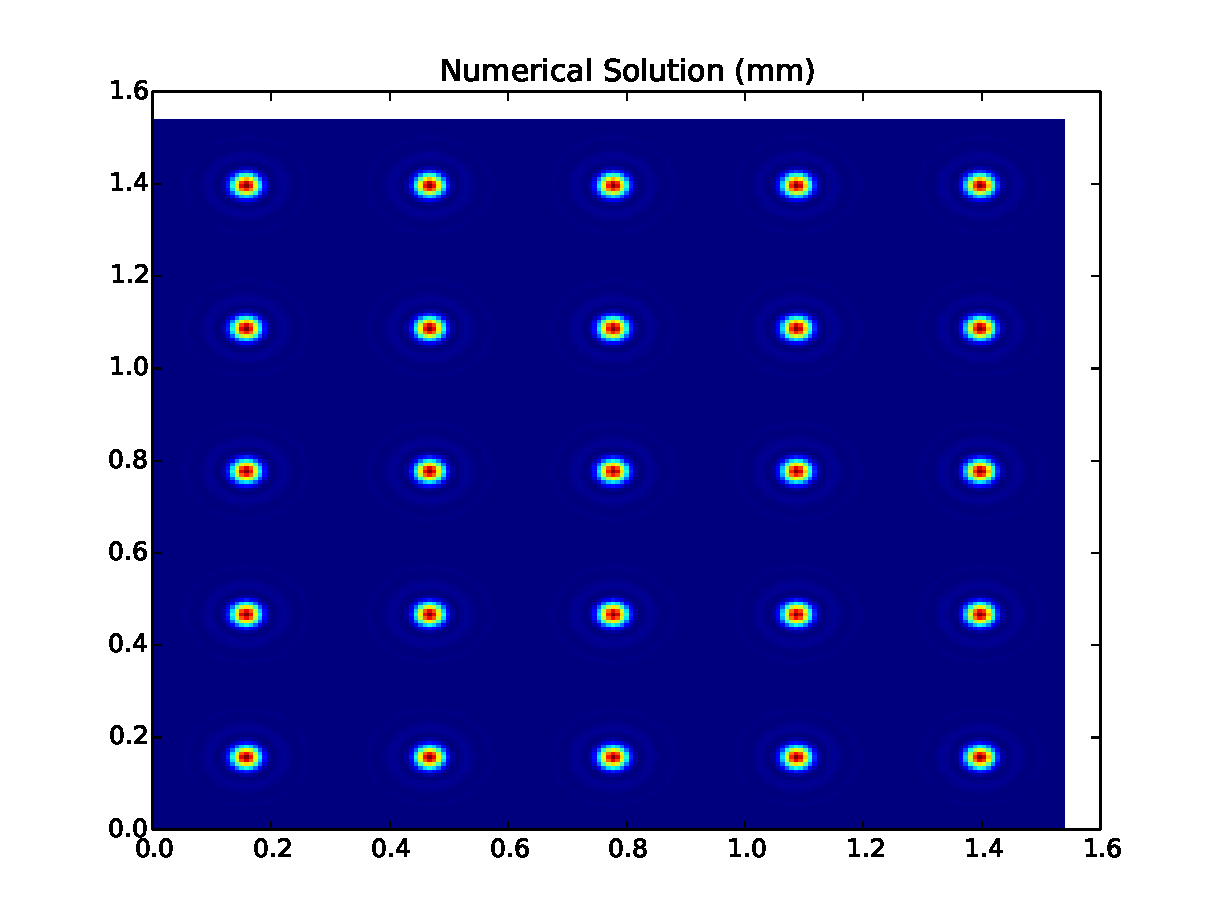
\includegraphics[width=.5\linewidth]{figures/NoNoise.pdf}
   	}
    \hfill
	\subfloat[Poisson noise]{%
    	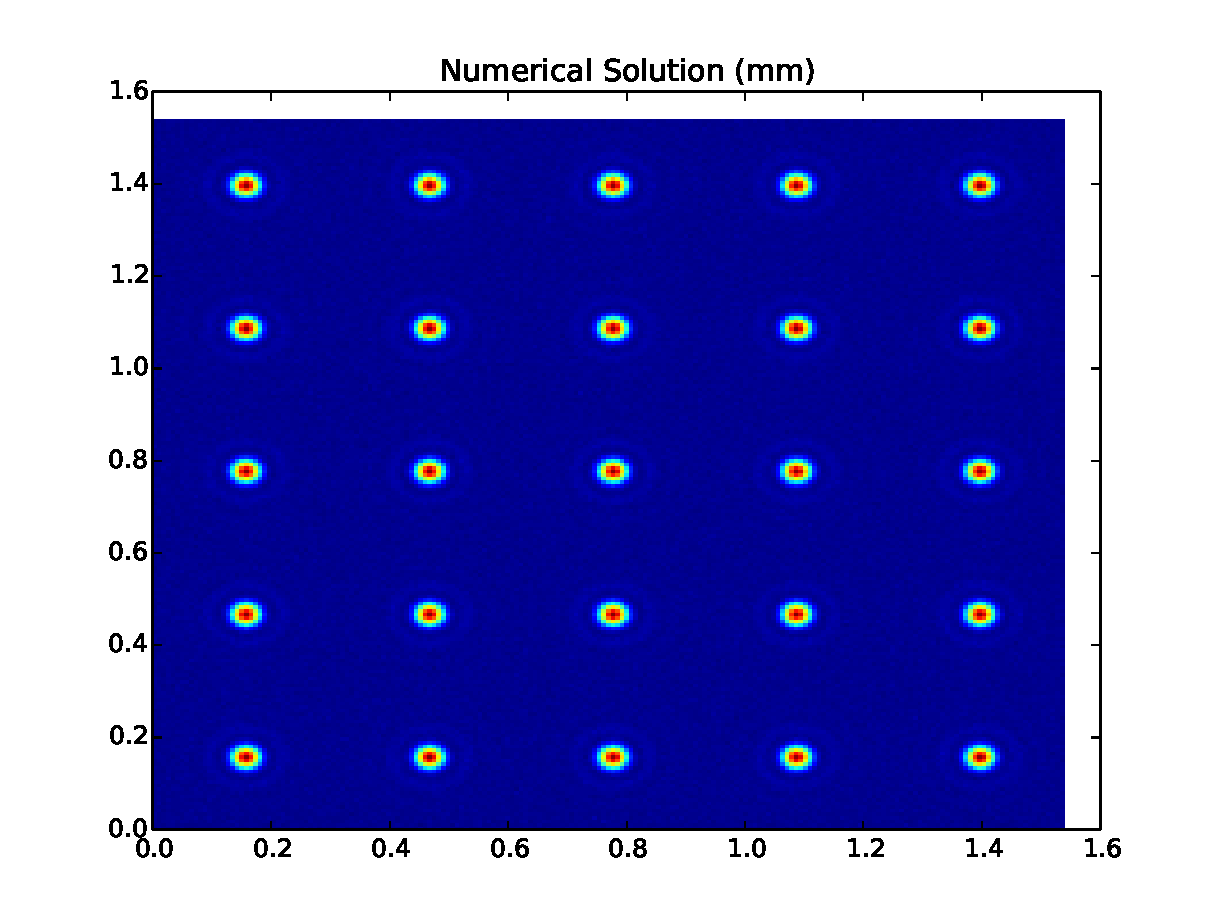
\includegraphics[width=.5\linewidth]{figures/PoissonNoise.pdf}
   	} \\
   	
    \subfloat[Readout noise with $\sigma_r = 0.005$]{%
    	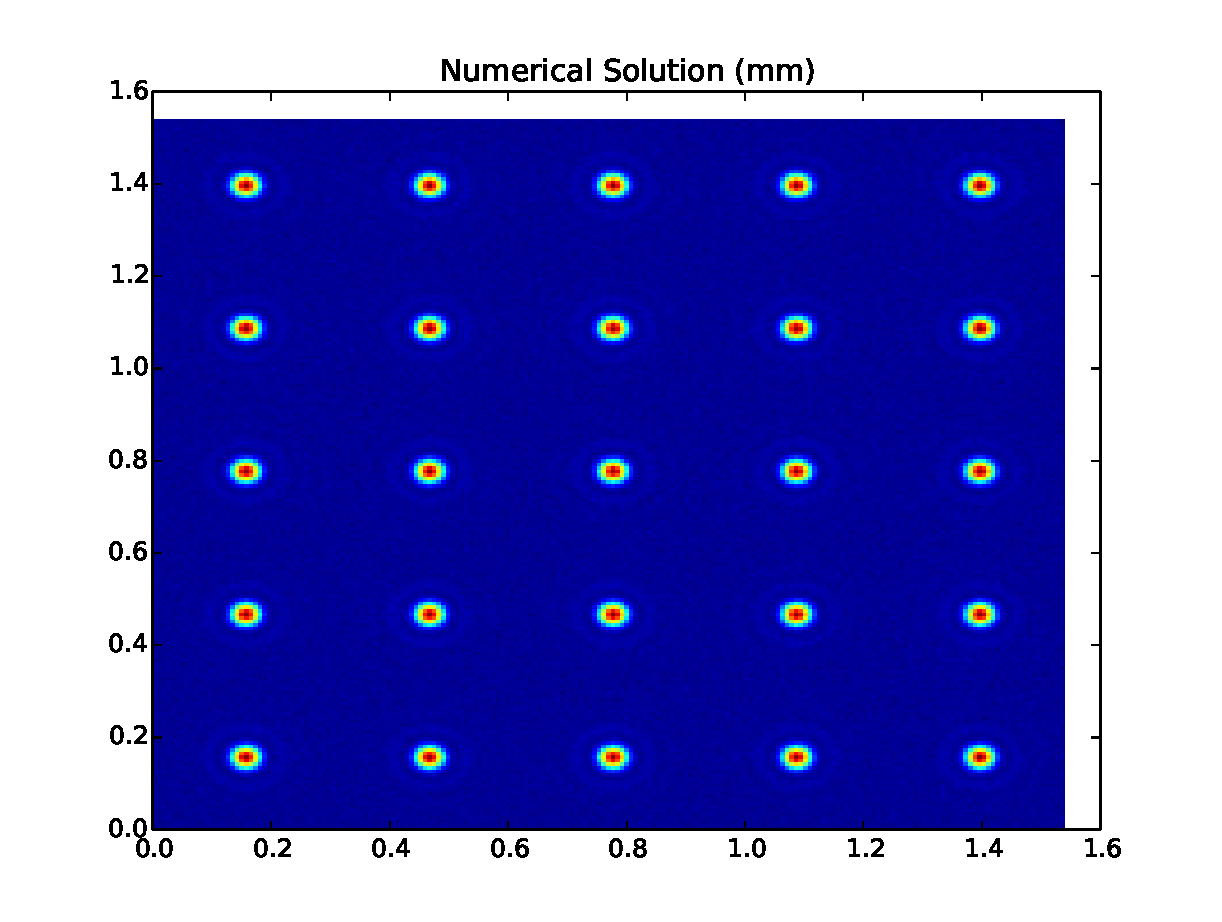
\includegraphics[width=.5\linewidth]{figures/ReadoutNoise.pdf}
   	}  
   	\hfill
	\subfloat[Poisson and Readout noise with $\sigma_r = 0.005$]{%
    	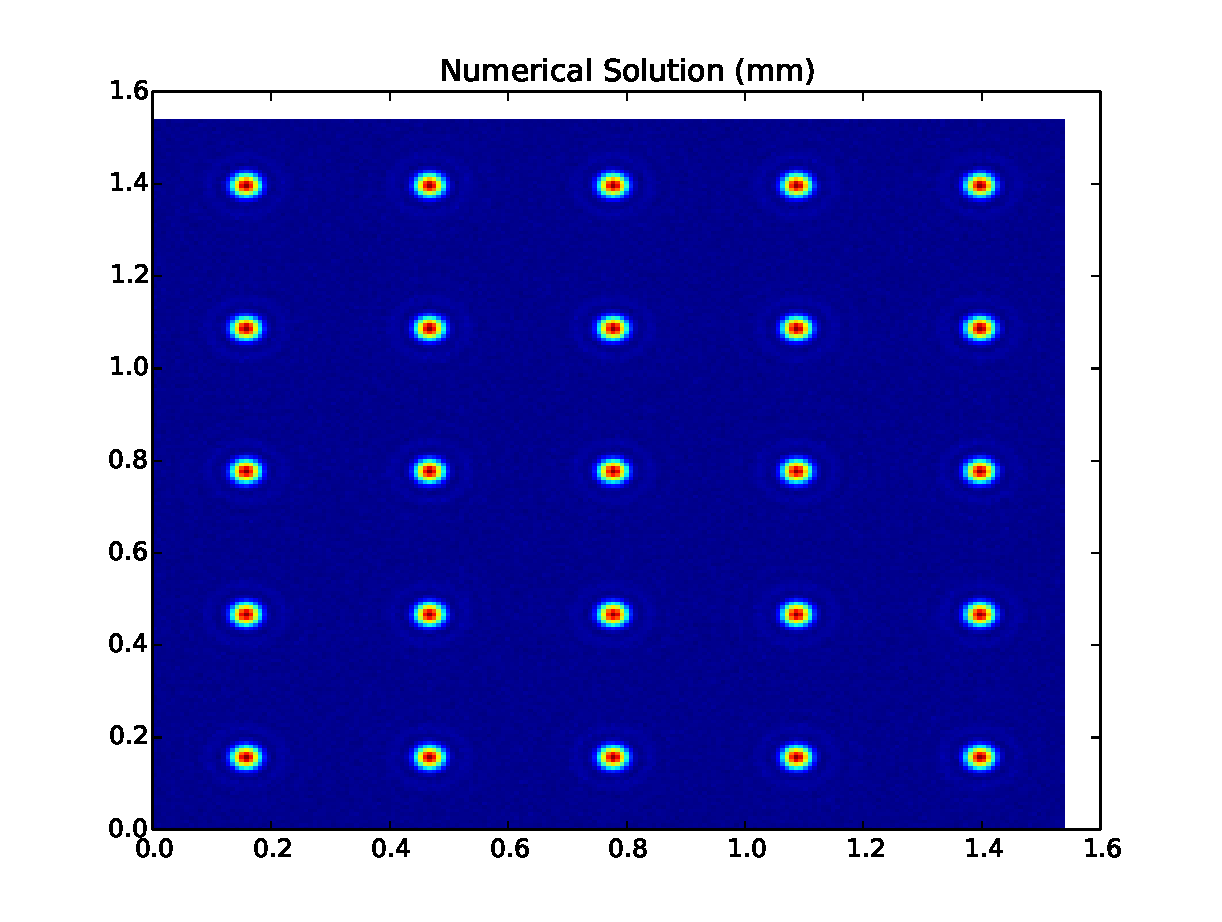
\includegraphics[width=.5\linewidth]{figures/MeasNoise.pdf}
   	}    
	\caption{Effect of Measurement Noise}
	\label{fig:MNoise}
\end{figure}